\chapter{\chatextlogicalReasoning}\label{cha:logicalReasoning}

We approach logical inference by defining probability distributions based on propositional formulas and then apply the methodology introduced in the more generic situation of probabilistic inference.
Logical approaches pay here special attention to situations of certainty, where a state of a variable has probability $1$.
In this situation, we say that the corresponding formula is entailed.
%Such situations are called entailment, and we will investigate how we can find these by contractions.

% From Probabilistic 
We start the discussion with the derivation of contraction criteria for logical entailment.
We interpret formulas by distributions and extend logical entailment towards probabilistic reasoning.
%This enables us to define logical entailment based on the resulting conditional distributions.

\sect{Entailment in Propositional Logics}

Entailment is the central consequence relation among logical formulas.
Let us define this relation first based on the models of a knowledge base and a test formula.

\begin{definition}[Entailment of propositional formulas]
    \label{def:logicalEntailment}
    Given two propositional formulas $\kb$ and $\exformula$ we say that $\kb$ entails $\exformula$, denoted by $\kb\models\exformula$, if any model of $\kb$ is also a model of $\exformula$, that is
    \begin{align*}
        \uniquantwrtof{\shortatomindicesin}{\imppremhead{\kbat{\indexedshortcatvariables}=1}{\formulaat{\indexedshortcatvariables}=1}} \, .
    \end{align*}
    If $\kb\models\lnot\exformula$ holds, we say that $\kb$ contradicts $\exformula$.
\end{definition}

% Connection with tensor formalism
To use the tensor network formalism for the decision of entailment, we will in the following develop three equivalent criteria for entailment. %, based on contractions.

\subsect{Deciding Entailment by contractions}

First of all, we can decide entailment based on vanishing contractions with the negated test formula.

\begin{theorem}[Contraction Criterion of Entailment]
    \label{the:contCriterionLogEntailment}
    We have $\kb\models\exformula$ if and only if
    \begin{align*}
        \contraction{\kb,\lnot\exformula} = 0 \, .
    \end{align*}
\end{theorem}
\begin{proof}
    \proofleftsymbol:
    If for a $\shortatomindicesin$ we have $\kbat{\indexedshortcatvariables}=1$ but not $\big(\exformulaat{\indexedshortcatvariables}=1\big)$, we would have $\big(\lnot\exformulaat{\indexedshortcatvariables}=1\big)$ and
    \begin{align*}
        \contraction{\kb,\lnot\exformula} =
        \sum_{\shortatomindicesin} \kbat{\indexedshortcatvariables} \cdot \exformulaat{\indexedshortcatvariables} > 1 \, .
    \end{align*}
    Thus, whenever the contraction vanishes, we have
    \begin{align*}
        \uniquantwrtof{\shortatomindicesin}{\imppremhead{\kbat{\indexedshortcatvariables}=1}{\formulaat{\indexedshortcatvariables}=1}} \, .
    \end{align*}
    %for all $\shortatomindicesin$ that $\big(\kbat{\indexedshortcatvariables}=1\big) \rightarrow \big(\formulaat{\indexedshortcatvariables}=1\big)$.

    \proofrightsymbol:
    Conversely, if the contraction $\contraction{\kb,\lnot\exformula}$ does not vanish, we would find $\shortatomindicesin$ with $\kbat{\indexedshortcatvariables}=1$ and $\lnot\formulaat{\indexedshortcatvariables}=1$, therefore $\formulaat{\indexedshortcatvariables}=0$.
    It follows that $\kb\models\exformula$ does not hold.
\end{proof}


% Can use relational encoding
The contraction criterion can be extended to the decision of contradiction as well, since $\kb\models\lnot\exformula$ is equivalent to $\sbcontraction{\kb,\exformula}=0$.
Therefore, entailment and contradiction can be decided simultaneously by a single contraction, as we state next.
%To decide whether a formula is entailed, or its negation is entailed (in which case one says that the formula is contradicted) by a single contraction, one can perform the contraction
%\begin{align*}
%	\hypercore = \sbcontractionof{\kbat{\shortcatvariables},\formulaat{\shortcatvariables,\exformulavar}}{\exformulavar}
%\end{align*}

\begin{theorem}
    \label{the:entailmentContradictionContraction}
    Given propositional formulas $\kb$ and $\exformula$ we build
    \begin{align*}
        \hypercoreat{\exformulavar}
        = \sbcontractionof{\kbat{\shortcatvariables},\formulaat{\shortcatvariables,\exformulavar}}{\exformulavar} \, .
    \end{align*}
    Then $\kb\models\exformula$ is equivalent to $\hypercoreat{\exformulavar=0}=0$, and $\kb\models\lnot\exformula$ is equivalent to $\hypercoreat{\exformulavar=1}=0$ \, .
\end{theorem}
\begin{proof}
    This follows from \theref{the:contCriterionLogEntailment} using that
    \begin{align*}
        \sbcontraction{\kb,\lnot\exformula} = \hypercoreat{\exformulavar=0}
    \end{align*}
    and
    \begin{align*}
        \sbcontraction{\kb,\exformula} = \hypercoreat{\exformulavar=1} \, .
    \end{align*}
\end{proof}





\subsect{Deciding Entailment by partial ordering}

% Subset relation
Logical entailment can be understood by subset relations of the models of the respective formulas.
This perspective can be applied with subset encodings in \charef{cha:basisCalculus}.
The subset relation corresponds with partial ordering of its encoded tensors, as will be shown in \theref{the:subsetRelationSubsetEncoding}.
For two propositional formulas, we denote to this end $\exformula\prec\secexformula$ (see \defref{def:partialOrder}), if and only if for all $\shortatomindicesin$
\begin{align*}
    \exformulaat{\indexedshortcatvariables} \leq \secexformulaat{\shortcatindices}  \, .
\end{align*}

\begin{theorem}[Partial Ordering Criterion of Entailment]
    \label{the:orderingEntailmentCriterion}
    We have $\kb\models\exformula$ if and only if $\kbat{\shortcatvariables}\prec\exformulaat{\shortcatvariables}$.
\end{theorem}
\begin{proof}
    Since both $\kb$ and $\exformula$ are boolean tensors, we have for any $\shortatomindicesin$ that
    \begin{align*}
        \kbat{\indexedshortcatvariables},\formulaat{\indexedshortcatvariables}\in\ozset \, .
    \end{align*}
    Thus,
    \begin{align*}
        \uniquantwrtof{\shortatomindicesin}{\kbat{\indexedshortcatvariables}\leq\formulaat{\indexedshortcatvariables}}
    \end{align*}
    is equivalent to
    \begin{align*}
        \uniquantwrtof{\shortatomindicesin}{\imppremhead{\kbat{\indexedshortcatvariables}=1}{\formulaat{\indexedshortcatvariables}=1}} \, .
    \end{align*}
    This states that $\kbat{\shortcatvariables}\prec\exformulaat{\shortcatvariables}$ is equivalent to $\kb\models\exformula$.
\end{proof}



\subsect{Redundancy of entailed formulas}

Another interpretation of entailment is by redundancy of a formula in a Knowledge Base.
This is especially interesting for the sparse representation of Knowledge Bases.
%Towards getting insights on this we first show that entailed formulas can be dropped from the Knowledge Base.

\begin{theorem}[Redundancy Criterion of Entailment]
    \label{the:ReduncancyOfEntailed}
    If and only if $\kb\models\exformula$ we have
    \begin{align*}
        \kbat{\shortcatvariables}= \contractionof{\kb,\exformula}{\shortcatvariables}  \, .
    \end{align*}
\end{theorem}
\begin{proof}
    For any formula $\exformula$ we have
    \begin{align*}
        \onesat{\shortcatvariables} = \exformulaat{\shortcatvariables} + \lnot\exformulaat{\shortcatvariables}
    \end{align*}
    and thus
    \begin{align*}
        \kbat{\shortcatvariables}
        & = \contractionof{\kbat{\shortcatvariables},\onesat{\shortcatvariables}}{\shortcatvariables} \\
        & = \contractionof{\kbat{\shortcatvariables},\exformulaat{\shortcatvariables}}{\shortcatvariables} +  \contractionof{\kbat{\shortcatvariables},\lnot\exformulaat{\shortcatvariables}}{\shortcatvariables} \, .
    \end{align*}
    Now, by \theref{the:contCriterionLogEntailment} we have $\kb\models\exformula$, if and only if $\contractionof{\kbat{\shortcatvariables},\lnot\exformulaat{\shortcatvariables}}{\shortcatvariables}=0$, which is thus equal to
    \begin{align*}
        \kbat{\shortcatvariables}
        = \contractionof{\kbat{\shortcatvariables},\exformulaat{\shortcatvariables}}{\shortcatvariables} \, .
    \end{align*}
\end{proof}

%This provides us with another interpretation of the entailment relation, in terms of redundant formulas.
%\begin{remark}[Sparsest Description of a Knowledge Base]
%	Given a set of worlds indexed by $\hypercore$, find the sparsest set of formulas $\kb$ such that
%		\[ \hypercore = {\kb} \]
%	would be benefitial for small computational complexity.
%	Since the formula tensors are invariant under entailment, we can drop entailed formulas.
%\end{remark}

\subsect{Contraction Knowledge Base}

We exploit the contraction and redundancy criteria of entailment to sketch an implementation of a propositional Knowledge Base in \algoref{alg:contractionKB}.
Here the function $\mathrm{ASK}(\exformula)$ returns, whether a formula $\exformula$ is entailed or contradicted by a Knowledge Base.
If the formula is neither entailed or contradicted, we say it is contingent.
If it is both, we have $\kbat{\shortcatvariables}=0$ and thus an inconsistent Knowledge Base.
Exploiting \theref{the:entailmentContradictionContraction} we decide these situations based on a single contraction.

The function $\mathrm{TELL}(\exformula)$ incorporates an additional formula $\exformula$ into a Knowledge Base $\kb$.
Here we exploit \theref{the:ReduncancyOfEntailed} and do not add a formula, which is entailed in order to maintain a sparse representation. %(in which case it returns Incons).
The function further refuses to add a formula, which would make the Knowledge Base inconsistent (returns Refused) and only changes the Knowledge Base in case of a contingent formula (returns Added).

% Works also for Markov Networks!
\begin{algorithm}[hbt!]
    \caption{Contraction Knowledge Base}\label{alg:contractionKB}
    ASK($\kb$, $\exformula$)
    \begin{algorithmic}
        \State{$\hypercoreat{\formulavar} \algdefsymbol \contractionof{\{\secexformulaat{\shortcatvariables} \, : \, \secexformula\in\kb\},\rencodingofat{\exformula}{\formulavar,\shortcatvariables}}{\formulavar}$}
        \If{$\hypercoreat{\formulavar=0}=0$ and $\hypercoreat{\formulavar=1}=0$ }
            \State{return Inconsistent}
        \EndIf
        \If{$\hypercoreat{\formulavar=0}=0$}
            \State{return Entailed}
        \EndIf
        \If{$\hypercoreat{\formulavar=1}=0$}
            \State{return Contradicted}
        \EndIf
        \State{return Contingent}
    \end{algorithmic}
    TELL($\kb$, $\exformula$)
    \begin{algorithmic}
        \State{answer $\algdefsymbol$ ASK($\exformula$)}
        \If{answer is Inconsistent:}
            \State{return Inconsistent}
        \EndIf
        \If{answer is Entailed:}
            \State{return Redundant}
        \EndIf
        \If{answer is Inconsistent or Contradicted:}
            \State{return Refused}
        \EndIf
        \If{answer is Inconsistent or Contradicted:}
            \State $\kb \algdefsymbol \kb\cup\{\exformula\}$
            \State{return Added}
        \EndIf
    \end{algorithmic}

\end{algorithm}



\sect{Formulas as Random Variables}

%\red{Aim here: Relate with the probabilistic reasoning concepts of marginal and conditional distributions.}
%\red{Given a probability distribution $\probtensor$ of atoms we add a variable by building the Markov Network of $\probtensor$ and $\rencodingof{\exformula}$ to get a joint distribution of the atoms and a query formula $\exformula$}

In order to present logical entailment as extreme cases of more generic probabilistic reasoning, we now provide probabilistic interpretations of propositional formulas.
% Interpretation of relational encoding as conditional probabilities
In the next sections, we will investigate two ways of interpreting relational encodings of formulas as conditional probabilities.
The atom centric one, which understands the atomic legs as conditions and calculates the truth of the formula, leads to a direct interpretation of $\rencodingof{\exformula}$ as a conditional probability distribution.
When instead taking the formula itself centric, we get uniform distributions of its models and the complement, when conditioning on the satisfaction of the formula.

\subsect{Probabilistic queries by formulas}

Let $\probat{\shortcatvariables}$ be a joint distribution of atomic variables $\catvariableof{\atomenumerator}$, where $\atomenumeratorin$, taking variables in $\catdimof{\atomenumerator}=2$.
Let us then ask a query in the formalism of \defref{def:queries}, where the query function is assumed to be a propositional formula.
The joint distribution can be extended to a variable $\exformulavar$ representing the satisfaction of a formula $\exformula$ given an assignment to the atoms, by adding its relational encoding as
\begin{align*}
    \probat{\exformulavar,\shortcatvariables}
    = \contractionof{\rencodingofat{\exformula}{\exformulavar,\shortcatvariables},\probat{\shortcatvariables}}{\shortcatvariables} \, .
\end{align*}
Let us note, that this is a normed probability distribution, since $\contractionof{\rencodingofat{\exformula}{\exformulavar,\shortcatvariables}}{\shortcatvariables}=\onesat{\shortcatvariables}$ and $\probat{\shortcatvariables}$ is normed.

Conditioning this probability distribution on the atoms, we get
\begin{align*}
    \condprobof{\formulavar}{\shortcatvariables}
    = \rencodingofat{\exformula}{\shortcatvariables} \, .
\end{align*}
We thus interpret the relational encoding of a formula as a conditional probability of $\exformula$ given the assignments to the atoms $\shortcatvariables$ and depict this by
\begin{center}
    \begin{tikzpicture}[scale=0.35,thick] % , baseline = -3.5pt



\draw[->-] (2,-1)--(2,1) node[midway,right] {\tiny $\formulavar$};

\draw (-3,-1) rectangle (7,-3);
\node[anchor=center] (text) at (2,-2) {\small $\condprobof{\formulavar}{\atomicformulas}$};
\draw[-<-] (0,-3)--(0,-5) node[midway,left] {\tiny $\catvariableof{0}$};
\draw[-<-] (1.5,-3)--(1.5,-5) node[midway,left] {\tiny $\catvariableof{1}$};
\node[anchor=center] (text) at (3,-4) {$\cdots$};
\draw[-<-] (4,-3)--(4,-5) node[midway,right] {\tiny $\catvariableof{\atomorder\shortminus1}$};


\node[anchor=center] (text) at (9,-2) {${=}$};


\begin{scope}[shift={(12,0)}]

\draw[->-] (2,-1)--(2,1) node[midway,right] {\tiny $\formulavar$};
\draw (-1,-1) rectangle (5,-3);
\node[anchor=center] (text) at (2,-2) {\small $\rencodingof{\exformula}$};
\draw[-<-] (0,-3)--(0,-5) node[midway,left] {\tiny $\catvariableof{0}$};
\draw[-<-] (1.5,-3)--(1.5,-5) node[midway,left] {\tiny $\catvariableof{1}$};
\node[anchor=center] (text) at (3,-4) {$\cdots$};
\draw[-<-] (4,-3)--(4,-5) node[midway,right] {\tiny $\catvariableof{\atomorder\shortminus1}$};

\node[anchor=center] (text) at (7,-5) {${\cdot}$};

\end{scope}


\end{tikzpicture}
\end{center}
To be more precise, we have for any $\shortcatindices$
\begin{align*}
    \condprobof{\formulavar}{\indexedshortcatvariables} =
    \begin{cases}
        \fbasisat{\formulavar} & \text{if} \quad \exformulaat{\indexedshortcatvariables} = 0 \text{, i.e. $\shortcatindices$ is not a model of $\exformula$} \\
        \tbasisat{\formulavar} & \text{if} \quad \exformulaat{\indexedshortcatvariables} = 1 \text{, i.e. $\shortcatindices$ is a model of $\exformula$}
    \end{cases} \, .
\end{align*}

% Interpretation of directionality as
Since the conditional query $\condprobof{\formulavar}{\shortcatvariables}$ provides an interpretation of $\rencodingof{\exformula}$ as a conditional probability, we interpret $\probat{\exformulavar}$ as a marginal distribution inherited by $\probat{\shortcatvariables}$.
This is also reflected in the fact that both $\condprobof{\formulavar}{\shortcatvariables}$ and $\rencodingofat{\exformula}{\exformulavar,\shortcatvariables}$ are directed, since the first is a normation by \defref{def:queries} and the second an relational encoding of a formula.
Probabilistic queries (see \defref{def:queries}), which functions are propositional formulas are thus answered by the satisfaction rate of a propositional formula given a joint distribution of the corresponding atoms.


%This trivialization is depicted as:
%\begin{center}
%	\begin{tikzpicture}[scale=0.35,thick] % , baseline = -3.5pt



\draw (1,1) rectangle (3,3);
\node[anchor=center] (text) at (2,2) {\small $\ones$};
\draw[->] (2,-1)--(2,1) node[midway,right] {\tiny $\formulavar$};

\draw (-1,-1) rectangle (5,-3);
\node[anchor=center] (text) at (2,-2) {\small $\rencodingof{\exformula}$};
\draw[<-] (0,-3)--(0,-5) node[midway,left] {\tiny $\catvariableof{0}$}; 
\draw[<-] (1.5,-3)--(1.5,-5) node[midway,left] {\tiny $\catvariableof{1}$}; 
\node[anchor=center] (text) at (3,-4) {$\cdots$};
\draw[<-] (4,-3)--(4,-5) node[midway,right] {\tiny $\catvariableof{\atomorder-1}$}; 


\node[anchor=center] (text) at (7,-2) {${=}$};

\begin{scope}[shift={(10,0)}]

\draw (1,1) rectangle (3,3);
\node[anchor=center] (text) at (2,2) {\small $\ones$};

\draw[->] (2,-1)--(2,1) node[midway,right] {\tiny $\formulavar$};
\draw (-1,-1) rectangle (5,-3);
\node[anchor=center] (text) at (2,-2) {\small $\condprobof{\formulavar}{\atomicformulaof{\atomenumerator}}$};
\draw[<-] (0,-3)--(0,-5) node[midway,left] {\tiny $\catvariableof{0}$}; 
\draw[<-] (1.5,-3)--(1.5,-5) node[midway,left] {\tiny $\catvariableof{1}$}; 
\node[anchor=center] (text) at (3,-4) {$\cdots$};
\draw[<-] (4,-3)--(4,-5) node[midway,right] {\tiny $\catvariableof{\atomorder\shortminus1}$}; 

\end{scope}

\node[anchor=center] (text) at (17,-2) {${=}$};

\begin{scope}[shift={(20,0)}]

\draw (-1,-1) rectangle (5,-3);
\node[anchor=center] (text) at (2,-2) {\small $\ones$};
\draw[<-] (0,-3)--(0,-5) node[midway,left] {\tiny $\catvariableof{0}$}; 
\draw[<-] (1.5,-3)--(1.5,-5) node[midway,left] {\tiny $\catvariableof{1}$}; 
\node[anchor=center] (text) at (3,-4) {$\cdots$};
\draw[<-] (4,-3)--(4,-5) node[midway,right] {\tiny $\catvariableof{\atomorder\shortminus1}$}; 

\node[anchor=center] (text) at (6,-5) {$.$};

\end{scope}


\end{tikzpicture}
%\end{center}

%% Conditional interpretation -> Formulas as conditional probability ("local")
%Our main interpretation understands each tuple of indices $\shortcatindices$ as conditions of a probability tensor.
%Since the satisfaction of a formula is determined by $\shortcatindices$,
%Given a truth assignment to the atomic variables $\atomicformulaof{\atomenumerator}$, that is a choice of indices $\atomlegindexof{\atomenumerator}$, the truth of the formula.


%\begin{theorem}\label{the:conditionByAtoms}
%	Given any distribution $\probat{\shortcatvariables}$ of atomic variables, we extend the joint distribution to a formula variable $\exformulavar$ by contraction with the relational encoding $\rencodingofat{\exformula}{\exformulavar,\shortcatvariables}$.
%	Then the relational encoding $\rencodingofat{\exformula}{\exformulavar,\shortcatvariables}$ coincides with the conditional probability of that formula conditioned on the atoms, that is
%	\begin{align*}
%		\rencodingofat{\exformula}{\shortcatvariables}
%		= \condprobof{\formulavar}{\shortcatvariables} \, .
%	\end{align*}
%	We depict this by
%	\begin{center}
%		\begin{tikzpicture}[scale=0.35,thick] % , baseline = -3.5pt



\draw[->] (2,-1)--(2,1) node[midway,right] {\tiny $\formulavar$};

\draw (-3,-1) rectangle (7,-3);
\node[anchor=center] (text) at (2,-2) {\small $\condprobof{\formulavar}{\atomicformulas}$};
\draw[<-] (0,-3)--(0,-5) node[midway,left] {\tiny $\catvariableof{0}$}; 
\draw[<-] (1.5,-3)--(1.5,-5) node[midway,left] {\tiny $\catvariableof{1}$}; 
\node[anchor=center] (text) at (3,-4) {$\cdots$};
\draw[<-] (4,-3)--(4,-5) node[midway,right] {\tiny $\catvariableof{\atomorder\shortminus1}$}; 


\node[anchor=center] (text) at (9,-2) {${=}$};


\begin{scope}[shift={(12,0)}]

\draw[->] (2,-1)--(2,1) node[midway,right] {\tiny $\formulavar$};
\draw (-1,-1) rectangle (5,-3);
\node[anchor=center] (text) at (2,-2) {\small $\rencodingof{\exformula}$};
\draw[<-] (0,-3)--(0,-5) node[midway,left] {\tiny $\catvariableof{0}$}; 
\draw[<-] (1.5,-3)--(1.5,-5) node[midway,left] {\tiny $\catvariableof{1}$}; 
\node[anchor=center] (text) at (3,-4) {$\cdots$};
\draw[<-] (4,-3)--(4,-5) node[midway,right] {\tiny $\catvariableof{\atomorder\shortminus1}$}; 

\node[anchor=center] (text) at (7,-5) {${\cdot}$};

\end{scope}


\end{tikzpicture}
%	\end{center}
%\end{theorem}
%\begin{proof}
%	The distribution $\probtensor$ does not influence the conditional query, since the normation acts on any state.
%
%\end{proof}

\subsect{Uniform distributions of the models}

% Defining probability distribution by formulas
Let us now converse the order of conditioning from $\condprobof{\exformulavar}{\shortcatvariables}$ to $\condprobof{\shortcatvariables}{\exformulavar}$.
In this way, we understand a propositional formula as a definition of a joint probability distributions of the atoms, instead of a formulation of a probabilistic query against a joint distribution.
To this end, we define by the single tensor core $\{\rencodingofat{\exformula}{\exformulavar,\shortcatvariables}\}$ a Markov Network $\probofat{\{\exformula\}\cup[\catorder]}{\exformulavar,\shortcatvariables}$.
%Given a Markov Network $\probtensor$ with a single core $\rencodingof{\exformula}$ for a propositional formula $\exformula$.
By definition we have
\begin{align*}
    \condprobwrtof{\{\exformula\}\cup[\catorder]}{\shortcatvariables}{\exformulavar}
    = \sbnormationofwrt{\rencodingof{\exformula}}{\shortcatvariables}{\exformulavar} \, .
\end{align*}
We depict this construction by:
\begin{center}
    \begin{tikzpicture}[scale=0.35,thick] % , baseline = -3.5pt


    \begin{scope}
        [shift={(-2,0)}]


        \draw[-<-] (2,-1)--(2,1) node[midway,right] {\colorlabelsize $\formulavar$};

        \draw (-1,-1) rectangle (5,-3);
        \node[anchor=center] (text) at (2,-2) {\corelabelsize $\condprobof{\atomicformulas}{\formulavar}$};
        \draw[->-] (0,-3)--(0,-5) node[midway,left] {\colorlabelsize $\catvariableof{0}$};
        \draw[->-] (1.5,-3)--(1.5,-5) node[midway,left] {\colorlabelsize $\catvariableof{1}$};
        \node[anchor=center] (text) at (3,-4) {$\cdots$};
        \draw[->-] (4,-3)--(4,-5) node[midway,right] {\colorlabelsize $\catvariableof{\atomorder\shortminus1}$};


        \node[anchor=center] (text) at (7,-2) {${=}$};

    \end{scope}


    \node[anchor=center] (text) at (8,-2.25) {$\sum\limits_{\headindexof{\exformula}\in[2]}$};

    \draw[] (10,-1) rectangle (12,-3);
    \node[anchor=center] (text) at (11,-2) {\corelabelsize $\onehotmapof{\headindexof{\exformula}}$};

    \draw[->-] (11,-3)--(11,-5) node[midway,right] {\colorlabelsize $\formulavar$};



    \begin{scope}
        [shift={(15,0)}]

        \draw[] (1,1) rectangle (3,3);
        \node[anchor=center] (text) at (2,2) {\corelabelsize $\onehotmapof{\headindexof{\exformula}}$};

        \draw[->-] (2,-1)--(2,0.5) node[right] {\colorlabelsize $\formulavar$};
        \drawvariabledot{2}{0}
        \draw (2,0.5) -- (2,1);
        \draw (-1,-1) rectangle (5,-3);
        \node[anchor=center] (text) at (2,-2) {\corelabelsize $\bencodingof{\exformula}$};
        \draw[-<-] (0,-3)--(0,-5) node[midway,left] {\colorlabelsize $\catvariableof{0}$};
        \draw[-<-] (1.5,-3)--(1.5,-5) node[midway,left] {\colorlabelsize $\catvariableof{1}$};
        \node[anchor=center] (text) at (3,-4) {$\cdots$};
        \draw[-<-] (4,-3)--(4,-5) node[midway,right] {\colorlabelsize $\catvariableof{\atomorder\shortminus1}$};


    \end{scope}


    \begin{scope}
        [shift={(25,0)}]

        \draw (-5,-7) -- (0,3);

        \draw[] (1,1) rectangle (3,3);
        \node[anchor=center] (text) at (2,2) {\corelabelsize $\onehotmapof{\headindexof{\exformula}}$};

        \draw[->-] (2,-1)--(2,0.5) node[right] {\colorlabelsize $\formulavar$};
        \drawvariabledot{2}{0}
        \draw (2,0.5) -- (2,1);
        \draw (-1,-1) rectangle (5,-3);
        \node[anchor=center] (text) at (2,-2) {\corelabelsize $\bencodingof{\exformula}$};
        \draw[-<-] (0,-3)--(0,-5) node[midway,left] {\colorlabelsize $\catvariableof{0}$};
        \draw[-<-] (1.5,-3)--(1.5,-5) node[midway,left] {\colorlabelsize $\catvariableof{1}$};
        \node[anchor=center] (text) at (3,-4) {$\cdots$};
        \draw[-<-] (4,-3)--(4,-5) node[midway,right] {\colorlabelsize $\catvariableof{\atomorder\shortminus1}$};

        \draw (-1,-5) rectangle (5,-7);
        \node[anchor=center] (text) at (2,-6) {\corelabelsize $\ones$};

    \end{scope}

    \node[anchor=center] (text) at (32,-5) {$.$};

\end{tikzpicture}
\end{center}

% Conditioning on the formula being true
Let us further investigate the slices of $\condprobof{\shortcatvariables}{\exformula}$ with respect to $\exformula$, which define distributions of the states of the factored system.
To this end, let us condition on the event of $\exformula=1$, for which we have the distribution
\begin{align}
    \label{eq:eventFormulaProb}
    \condprobof{\shortcatvariables}{\formulavar=1} = \frac{1}{\sbcontraction{\exformula}}
    \sum_{\shortatomindicesin \, : \, \formulaat{\indexedshortcatvariables}=1} \onehotmapofat{\shortcatindices}{\shortcatvariables} \, .
\end{align}
With $\sbcontraction{\exformula}$ being the number of models of $\exformula$, this is the uniform distribution among the models of $\exformula$.
Conversely, when conditioning on the event $\formulavar=0$ we get a uniform distribution of the models of $\lnot\exformula$.

% 
The probability distribution in Equation~\eqref{eq:eventFormulaProb} is well defined except for the case that $\sbcontraction{\exformula}=0$.
In that case we would have $\exformulaat{\shortcatvariables}=\zerosat{\shortcatvariables}$ and call $\exformula$ unsatisfiable, since it has no models.

%% Uniform interpretation -> KB as probability distribution over its models ("global")
From an epistemological point of view, probability theory is a generalization of logics, since we allow for probability values in the interval $[0,1]$.
The set of distributions being constructed by conditioning on propositional formulas as in Equation~\eqref{eq:eventFormulaProb} correspond within the set of probability distributions with those being constant on their support.
% More specific
While the distributions build a $2^\atomorder-1$-dimensional manifold, the formulas parametrize by this construction $2^{\left(2^\atomorder\right)}$.%, most of which having vanishing coordinates.




\subsect{Probability of a formula given a Knowledge Base}

% Both directions for entailment
We now combine the ideas of the previous two subsections and define probabilities of formulas $\exformula$ given the satisfaction of another formula $\kb$, which we call a knowledge base.
We have % by \theref{the:conditionByAtoms} % Again, Markov Network with rencoding of \exformula, \kb build the precise \probtensor
\begin{align*}
    \condprobof{\formulavar}{\kbvar}
    & = \sbcontractionof{
        \condprobof{\formulavar}{\atomicformulas}, \condprobof{\atomicformulas}{\kbvar}
    }{\formulavar,\kbvar} \\
    & = \sbnormationofwrt{\rencodingof{\exformula},\rencodingof{\kb}}{\formulavar}{\kbvar} \, .
\end{align*}
We notice, that we have to assume a satisfiable knowledge base $\kb$ for this construction to be well-defined.

% 
Of special interest is the conditional probability of $\formulavar$ given that $\kbvar$ is satisfied, that is
\begin{align*}
    \condprobof{\formulavar}{\kbvar=1}
    & = \normationof{\{\rencodingof{\exformula} ,\kb\}}{\formulavar}\\
    & = \frac{\contractionof{\{\rencodingof{\exformula},\kb\}}{\formulavar}}{\contraction{\{\kb\}}} \, .
\end{align*}
This conditional probability establishes a connection with the entailment relation of propositional formulas, as we show next.

%
\begin{theorem}
    \label{the:probEntailment}
    Given a satisfiable formula $\kb$, we have $\kb\models\exformula$, if and only if
    \begin{align*}
        \condprobof{\formulavar=0}{\kbvar=1} = 0 \, .
    \end{align*}
\end{theorem}
\begin{proof}
    Since $\kb$ is satisfiable, we have $\sbcontraction{\kb}>0$ and
    \[ \condprobof{\formulavar=0}{\kbvar=1} = \frac{\sbcontraction{\lnot\exformula,\kb}}{\sbcontraction{\kb}} \, .  \]
    This term vanishes if and only if $\sbcontraction{\lnot\exformula,\kb}$ vanish.
    Now, by \theref{the:contCriterionLogEntailment} we have $\kb\models\exformula$ if and only if $\contraction{\kb,\lnot\exformula}=0$, which is therefore equal to $\condprobof{\formulavar=0}{\kbvar=1}=0$.
\end{proof}

Since any conditional distribution is directed, we have
\begin{align}
    \condprobof{\formulavar}{\kbvar=1} = %\begin{cases}
    \fbasisat{\formulavar}  & \text{if} \quad \kb\models\lnot\exformula \\
    \tbasisat{\formulavar}  & \text{if} \quad \kb\models\exformula \\
    %\tbasis & \text{if }\kb \models \exformula \\
    \notin \{\fbasisat{\formulavar},\tbasisat{\formulavar}\} & \text{else}
    \, .
\end{align}
We depict the case of entailment $\kb\models\exformula$ by the contraction diagram
%It suffices to check, whether the contraction with the normed Knowledge Base is the basis vector $\tbasis$, respectively $\fbasis$, that is
\begin{center}
    \begin{tikzpicture}[scale=0.35,thick]

\draw[->-] (2,-1)--(2,1) node[midway,right] {\tiny $\exformulavar$};
\draw (-1,-1) rectangle (5,-3);
\node[anchor=center] (text) at (2,-2) {\small $\bencodingof{\exformula}$};
\draw[-<-] (0,-3)--(0,-5) node[midway,left] {\tiny $\catvariableof{0}$};
\draw[-<-] (1.5,-3)--(1.5,-5) node[midway,left] {\tiny $\catvariableof{1}$};
\node[anchor=center] (text) at (3,-4) {$\cdots$};
\draw[-<-] (4,-3)--(4,-5) node[midway,right] {\tiny $\catvariableof{\atomorder\shortminus1}$};

\draw (-1.5,-5) rectangle (5.5,-7);
\node[anchor=center] (text) at (2,-6) {\small $\normalizationof{\kb}{\shortcatvariables}$};

\node[anchor=center] (text) at (9,-4) {\small ${=}$};

\draw[->-] (13,-3)--(13,-1) node[midway,right] {\tiny $\exformulavar$};
\draw (12,-5) rectangle (14,-3);
\node[anchor=center] (text) at (13,-4) {\small $\tbasis$};

\node[anchor=center] (text) at (16,-6) {$\cdot$};

\end{tikzpicture}
\end{center}

We can further omit the normation by $\sbcontraction{\kb}$ when deciding entailment, and thus drop the assumption of satisfiability of $\kb$, as we state next.

% Not needed?
\begin{theorem}
    Given a formula $\kb$, we have $\kb\models\exformula$ (respectively $\kb\models\lnot\exformula$), if and only if
    \begin{align*}
        \sbcontractionof{\kb,\rencodingof{\exformula}}{\formulavar=0} = 0
        \quad \text{( respectively }
        \sbcontractionof{\kb,\rencodingof{\exformula}}{\formulavar=1} = 0 \, .
    \end{align*}
\end{theorem}
\begin{proof}
    This follows from \theref{the:contCriterionLogEntailment} using that
    \begin{align*}
        \rencodingofat{\exformula}{\exformulavar=0,\shortcatvariables} = \lnot\exformulaat{\shortcatvariables} \quad \text{and} \quad \rencodingofat{\exformula}{\exformulavar=1,\shortcatvariables} = \exformulaat{\shortcatvariables} \, .
    \end{align*}
\end{proof}


%
Relating entailment to probability distributions motivates an extension of the entailment provided by \defref{def:logicalEntailment} to arbitrary probability distributions.

\begin{definition}
    \label{def:probEntailment}
    For any propositional formula $\exformulaat{\shortcatvariables}$ we say that a probability distribution $\probof{\shortcatvariables}$ probabilistically entails $\exformula$, denoted as $\probtensor\models\exformula$, if
    \begin{align*}
        \sbcontractionof{\probat{\shortcatvariables},\rencodingofat{\exformula}{\exformulavar,\shortcatvariables}}{\exformulavar=0} = 0 .
    \end{align*}
    If $\probtensor\models\lnot\exformula$, that is $\sbcontractionof{\probat{\shortcatvariables},\rencodingofat{\exformula}{\exformulavar,\shortcatvariables}}{\exformulavar=1} = 0$, we say that $\probtensor$ probabilistically contradicts $\exformula$.
\end{definition}

%
We note, that when choosing for a formula $\kb$ the uniform distribution
\begin{align*}
    \probat{\shortcatvariables}=\sbnormationof{\shortcatvariables}{\kbvar=1}
\end{align*}
among its models, then probabilistic entailment $\probtensor\models\exformula$ of a propositional formula $\exformula$ is by \theref{the:probEntailment} equivalent to $\kb\models\exformula$.

\subsect{Knowledge Bases as Base Measures for Probability Distributions}

% Generic Probability Tensors
Let us now further relate the probabilistic entailment provided by \defref{def:probEntailment} with logical entailment, by constructing a corresponding propositional formula to an arbitrary distribution.
Given a generic probability distribution $\probtensor$ we can build a Knowledge Base by
\begin{align*}
    \kb^{\probtensor} = \nonzerofunction \circ \probtensor \, ,
\end{align*}
where $\nonzerofunction:\rr\rightarrow \rr$ denotes the indicator function of the support defined as
\begin{align}
    \nonzeroof{x}
    = \begin{cases}
          0 & \text{if} \quad x=0 \\
          1 & \text{else}
    \end{cases} \, .
\end{align}

Probabilistic entailment with respect to $\probtensor$ is then equivalent to entailment with respect to $\kb^{\probtensor}$, as we show next.

% Generic case of distributions
\begin{theorem}
    \label{the:entailmentProbToLogical}
    Any probability distribution $\probat{\shortcatvariables}$ probabilistically entails a formula $\exformulaat{\shortcatvariables}$, if and only if $\kb^{\probtensor}\models\exformula$.
\end{theorem}
\begin{proof}
    Whenever $\probtensor$ does not entail $\exformula$ probabilistically we find a state $\shortatomindicesin$ such that
    \begin{align*}
        \probat{\indexedshortcatvariables} >0 \quad\text{and} \quad \formulaat{\indexedshortcatvariables} = 0 \, .
    \end{align*}
    We further have $\probat{\indexedshortcatvariables}>0$ if and only if $\kb^{\probtensor}[\indexedshortcatvariables]=1$.
    Therefore the statement
    \begin{align*}
        \imppremhead{\kb^{\probtensor}[\indexedshortcatvariables]=1}{\formulaat{\indexedshortcatvariables}=1}
    \end{align*}
    is not satisfied.
    Together, $\probtensor\models\exformula$ does not holds if and only if
    \begin{align*}
        \uniquantwrtof{\shortatomindicesin}{\imppremhead{\kb^{\probtensor}[\indexedshortcatvariables]=1}{\formulaat{\indexedshortcatvariables}=1}}
    \end{align*}
    is not satisfied.
    Therefore, probabilistic entailment of $\exformula$ by $\probtensor$ is equivalent to logical entailment of $\exformula$ by $\kb^{\probtensor}$.
\end{proof}

Let us use this to connect the entailment formalism with the representability (see \defref{def:representationBaseMeasure}) and positivity (see \defref{def:positivityBaseMeasure}) of distributions with respect to boolean base measures.

\begin{theorem}
    \label{the:minimalRepPosBaseMeasure}
    Let $\probtensor$ be a distribution of boolean variables and let $\basemeasure$ be a boolean base measure.
    Then, $\probtensor$ is representable with respect to $\basemeasure$, if and only if $\nonzerocirc\probtensor\models\basemeasure$.
    Further, $\probtensor$ is positive with respect to $\basemeasure$, if and only if $\basemeasure=\nonzerocirc\probtensor$.
\end{theorem}
\begin{proof}
    To show the first claim, let $\probtensor$ be a distribution and $\basemeasure$ be a base measure.
    With \defref{def:representationBaseMeasure}, $\probtensor$ is representable with respect to $\basemeasure$, if and only if
    \begin{align*}
        \uniquantwrtof{\shortatomindicesin}{\imppremhead{\basemeasureat{\indexedshortcatvariables}=0}{\probat{\indexedshortcatvariables}=0}}
    \end{align*}
    This is equal to
    \begin{align*}
        \uniquantwrtof{\shortatomindicesin}{\imppremhead{\nonzerocirc\probat{\indexedshortcatvariables}=1}{\basemeasureat{\indexedshortcatvariables}=1}}
    \end{align*}
    and by definition \defref{def:logicalEntailment} equal to $\basemeasure\models\nonzerocirc\probtensor$.

    To proof the second claim, we show that when $\probtensor$ is in addition positive with respect to $\basemeasure$, then also $\basemeasure\models\nonzerocirc\probtensor$ and thus $\basemeasure=\nonzerocirc\probtensor$.
    Let $\probtensor$ be a distribution, which is representable with respect to $\basemeasure$.
    Then $\probtensor$ is positive with respect to $\basemeasure$, if and only if
    \begin{align*}
        \uniquantwrtof{\shortatomindicesin}{\imppremhead{\basemeasureat{\indexedshortcatvariables}=1}{\probat{\indexedshortcatvariables}>0}}
    \end{align*}
    This is equal to
    \begin{align*}
        \uniquantwrtof{\shortatomindicesin}{\imppremhead{\basemeasureat{\indexedshortcatvariables}=1}{\nonzerocirc\probat{\indexedshortcatvariables}=1}}
    \end{align*}
    and thus $\basemeasure\models\nonzerocirc\probtensor$.
\end{proof}


\sect{Constraint Satisfaction Problems}

Let us now explore a more general class of logical inference problems and discuss probabilistic entailment within that class.
We then provide further examples based on categorical constraints.
Following Chapter~5 in \cite{russell_artificial_2021}, we now define Constraint Satisfaction Problems.

\begin{definition}
    Let there be a hypergraph $\graph=(\nodes,\edges)$ and $\extnet$ be a tensor network of boolean constraint tensors $\hypercoreofat{\edge}{\catvariableof{\edge}}$ to each $\edgein$, that is
    \begin{align*}
        \extnet = \{ \hypercoreofat{\edge}{\catvariableof{\edge}} \, : \, \edge\in\edges \} \, .
    \end{align*}
    The Constraint Satisfaction Problem (CSP) to $\extnet$ is the decision whether there is a state $\catindexof{\nodes}$ such that
    \begin{align*}
        \contractionof{\extnet}{\indexedcatvariableof{\nodes}} = 1 \, .
    \end{align*}
    We say the CSP is satisfiable, when there is such a state, and unsatisfiable if not.
\end{definition}

\subsect{Deciding entailment on Markov Networks}

Deciding entailment on Markov Networks is a general class of contraint satisfaction problems.
Here, any factor tensor in the Markov Networks produces a constraint tensor in the respective CSP.

\begin{theorem}
    \label{the:factorReduction}
    Let $\probof{\graph}$ be a Markov Network to the Tensor Network $\extnet=\extnetasset$ on a hypergraph $\graph=(\nodes,\edges)$. % $\secnodes\subset\nodes$ be a subset and
%	\begin{align*}
%		\probat{\catvariableof{\secnodes}} = \normationof{\{\hypercoreat{\edge} \, : \, \edge\in\edges \}}{\catvariableof{\secnodes}}
%	\end{align*}
    For each $\edge\in\edges$ we build the factor constraint cores
    \begin{align*}
        \sechypercoreofat{\edge}{\catvariableof{\edge}} = \nonzerocirc\hypercoreofat{\edge}{\catvariableof{\edge}} \, .
    \end{align*}
    Let further $\exformulaat{\catvariableof{\secnodes}}$ be a formula depending on the variables $\secnodes$, and build $\secgraph=(\nodes,\edges\cup\{\secnodes\})$.
    Then we have that $\probof{\graph}\models\exformula$ if and only if the constraint satisfaction problem of $\secgraph$ to the constraint tensors
    \begin{align*}
        \{\sechypercoreof{\edge} \, : \, \edge\in\edges \} \cup \{\lnot\exformula \}
    \end{align*}
    is unsatisfiable.
    %and
    %	\[ \tilde{\probtensor}[\catvariableof{\secnodes}] = \normationof{\{\nonzerofunction \circ \hypercoreat{\edge} \, : \, \edge\in\edges \}}{\catvariableof{\secnodes}} \]
    %Then we have for any $\exformula$ that $\probtensor\models\exformula$ if and only if $\tilde{\probtensor}\models\exformula$.
\end{theorem}
\begin{proof}
    We first show, that
    \begin{align*}
        \nonzerocirc\probofat{\graph}{\nodevariables} =
        \contractionof{\{\sechypercoreof{\edge} \, : \, \edge\in\edges \}}{\nodevariables} \, . %\nonzerocirc\tilde{\probtensor} \, .
    \end{align*}
    To this end, let $\catindexof{\nodes}\in\nodestatesof{\nodes}$ be arbitrary.
    We have $\probofat{\graph}{\indexednodevariables}=0$ if and only if at there is an edge $\edge\in\edges$ with $\hypercoreofat{\edge}{\indexedcatvariableof{\edge}}$.
    But this is equivalent to
    \begin{align*}
        \contractionof{\{\sechypercoreof{\edge} \, : \, \edge\in\edges \}}{\nodevariables} \, .
    \end{align*}
    We thus have for any $\catindexof{\nodes}\in\nodestatesof{\nodes}$
    \begin{align*}
        \nonzerocirc\probofat{\graph}{\indexednodevariables} =
        \contractionof{\{\sechypercoreof{\edge} \, : \, \edge\in\edges \}}{\indexednodevariables} \, . %\nonzerocirc\tilde{\probtensor} \, .
    \end{align*}

    To continue, we have $\probof{\graph}\models\exformula$ if and only if
    \begin{align*}
        \contraction{\extnetat{\shortcatvariables},\lnot\exformulaat{\shortcatvariables}} = 0
    \end{align*}
    which is equal to
    \begin{align*}
        \contraction{\nonzerocirc\extnetat{\shortcatvariables},\lnot\exformulaat{\shortcatvariables}} = 0 \, .
    \end{align*}
    We notice, that this is the unsatisfiability of the claimed Constraint Satisfaction Problem.

%	We first show
%	\begin{align}\label{eq:proofFacReduction}
%		 \nonzerocirc\probtensor = \nonzerocirc\tilde{\probtensor} \, .
%	\end{align}
%	The claim follows then from \theref{the:entailmentProbToLogical}.
%	To show \eqref{eq:proofFacReduction} let there be $\indexedcatvariableof{\secnodes}$ such that $\probtensor[\indexedcatvariableof{\secnodes}]=0$.
%	Then for any $\indexedcatvariableof{\nodes}$ extending  $\indexedcatvariableof{\secnodes}$ we have $\contractionof{\{\hypercoreat{\edge} \, : \, \edge\in\edges \}}{\indexedcatvariableof{\nodes}} = 0$ and thus also $\contractionof{\{\nonzerocirc\hypercoreat{\edge} \, : \, \edge\in\edges \}}{\indexedcatvariableof{\nodes}} = 0$ and $\tilde{\probtensor}[\indexedcatvariableof{\secnodes}]=0$.
%	One can similarly show, that when $\tilde{\probtensor}[\indexedcatvariableof{\secnodes}]=0$ then also ${\probtensor}[\indexedcatvariableof{\secnodes}]=0$.
%	The support of the distributions $\probtensor$ and $\tilde{\probtensor}$ is thus identical and \eqref{eq:proofFacReduction} holds.
\end{proof}

% Consequence: Reduction of probabilitic entailment to logical entailment.
For any positive tensor $\hypercore$ we have
\[ \nonzerocirc\hypercoreat{\catvariableof{\edge}} = \onesat{\catvariableof{\edge}} \, , \]
which does not influence the distribution and can be omitted from the Markov Network.
By \theref{the:factorReduction}, when deciding entailment, we can reduce all tensors of a Markov Network to their support and omit those with full support.
Since the support indicating tensors $\nonzerocirc\hypercoreat{\catvariableof{\edge}}$ are boolean, each is a propositional formula and the Markov Network is turned into a Knowledge Base of their conjunctions.
Deciding probabilitic entailment is thus traced back to logical entailment.

%Exponential families
Exponential families have a tensor network representation by a Markov Network (see \theref{the:expFamilyTensorRep}).
However, all factors corresponding with a coordinate of the statistic $\sstat$ have a trivial support, and therefore do not influence the support of the distribution.
The only tensors with non-trivial support are those to the boolean base measure $\basemeasure$.


\subsect{Categorical Constraints}\label{sec:categoricalTN}

%% Categorical variables with more possibilities
We so far in this chapter made the assumption that all categorical variables in factored systems to be represented by propositional logics take binary values (i.e. $\catdim=2$).
In cases where a categorical variable $\catvariable$ takes multiple values we define for each $\catindex$ an atomic formula $\catvariableof{\catindex}$ representing whether $\catvariable$ is assigned by $\catindex$ in a specific state.
%\[ \catvariableof{\catindex} =  (\catvariable = \catindex \, . \] Confusing notation
Following this construction we have the constraint that exactly one of the atoms $\catvariableof{\catindex}$ is $1$ at each state.

%% Capture constraint
%To capture the constraints resulting from this construction we introduce auxiliary parts. % of Bayesian Propositional Networks.
%Such constraints can also be expressed by a formula but would result in an unnecessary large tensor network.


%% Categorical selection map
\begin{definition}[Categorical Constraint and Atomization Variables]
    Given a list $\catvariableof{0},\ldots,\catvariableof{\catdim-1}$ of boolean variables and a categorical variable $\catvariable$ with dimension $\catdim$ a categorical constraint is a tensor $\categoricalmap[\catvariable,\catvariableof{[\catdim]}]$ defined as
    \begin{align*}
        \categoricalmapat{\indexedcatvariableof{[\catdim]},\indexedcatvariable}
%		 \categoricalmap(\catindex,\catindexof{\variableset})
        = \begin{cases}
              1 & \text{if} \quad \catindexof{[\catdim]} = \onehotmapof{\catindex} \quad \Big(\text{i.e. }\forall \catenumerator\in[\catdim] \big(\catindex=\catenumerator\big) \Leftrightarrow \big(\catindexof{\catenumerator}=1\big) \Big)\\
              0 & \text{else} \, .
        \end{cases}
    \end{align*}
    We then call the variables  $\catvariableof{0},\ldots,\catvariableof{\catdim-1}$ the atomization variables to the categorical variable $\catvariable$.
\end{definition}

%% Decomposition
With \theref{the:functionDecompositionBasisCP} the relational encoding $\categoricalcore$ decomposes in a basis $\cpformat$ format (see \figref{fig:CategoricalDecomposition}b) of if its coordinate maps $\categoricalmapof{\catenumerator}$, where $\catenumerator\in[\catdim]$, defined as
\begin{align*}
    \categoricalmapofat{\catenumerator}{\indexedcatvariableof{\catenumerator},\indexedcatvariable}
    = \begin{cases}
          1 & \text{if} \quad \catindex=\catenumerator \\
          0 & \text{else} \, .
    \end{cases}
\end{align*}
Their relational encoding are decomposed as
\begin{align}
    \categoricalcoreofat{\catenumerator}{\catvariableof{\catenumerator},\catvariable}
    = \onehotmapofat{1}{\catvariableof{\catenumerator}} \otimes \onehotmapofat{\catenumerator}{\catvariable}
    + \onehotmapofat{0}{\catvariableof{\catenumerator}} \otimes \big(\onesat{\catvariable}- \onehotmapofat{\catenumerator}{\catvariable}\big) \, .
\end{align}
We further have by \theref{the:functionDecompositionBasisCP}
\begin{align*}
    \rencodingofat{\categoricalmap}{\catvariableof{[\catdim]},\catvariable}
    = \contractionof{\{\categoricalcoreofat{\catenumerator}{\catvariableof{\catenumerator},\catvariable} \, : \, \catindex\in[\catdim]\}}{\catvariable, \catvariableof{0}, \ldots, \catvariableof{\catdim-1}} \, .
\end{align*}


In the next theorem we show how a categorical constraint can be enforced in a tensor network by adding the tensor $\categoricalmap$ to a contraction.

\begin{theorem}
    For any tensor $\hypercoreat{\shortcatvariables}$ and a categorical constraint defined by an ordered subset $\catvariableof{\variableset}\subset\shortcatvariables$, a variable $\catvariable\in\shortcatvariables$ we have
    \begin{align*}
        \contractionof{\hypercoreat{\shortcatvariables},\categoricalmapat{\catvariableof{\variableset},\catvariable}}{\indexedcatvariables}
        = \begin{cases}
              \hypercoreat{\indexedcatvariables} & \text{if} \quad \catindexof{\variableset} = \onehotmapof{\catindex} \\
              0 & \text{else} \, .
        \end{cases}
    \end{align*}
    Here by $\catindexof{\variableset}$ we denote the restriction of $\shortcatindices$ on the set $\variableset$.
\end{theorem}
\begin{proof}
    For any $\catindexof{[\atomorder]}$ we have
    \[ \contractionof{\{\hypercoreat{\shortcatvariables}, \categoricalmap\}}{\indexedcatvariables}  =
    \hypercoreat{\shortcatindices} \cdot \categoricalmap[\indexedcatvariableof{\variableset},\indexedcatvariable] \, .
    \]
    If $\catindexof{\variableset} = \onehotmapof{\catindex}$ we have $\categoricalmap[\indexedcatvariableof{\variableset},\indexedcatvariable] = 1$ and thus
    \[ \contractionof{\hypercoreat{\shortcatvariables},\categoricalmap}{\indexedcatvariables}  =  \hypercoreat{\shortcatindices}  \, . \]
    If $\catindexof{\variableset} \neq \onehotmapof{\catindex}$ then $\categoricalmap[\indexedcatvariableof{\variableset},\indexedcatvariable] = 0$ and
    \[ \contractionof{\hypercoreat{\shortcatvariables},\categoricalmap}{\indexedcatvariables}  = 0 \, . \]
\end{proof}

\begin{figure}[h]
    \begin{center}
        \begin{tikzpicture}[scale=0.35, thick] % , baseline = -3.5pt

\begin{scope}[shift={(-15,2)}]

\node[anchor=center] (text) at (-1,3) {${a)}$};


\node [circle, draw, thick, fill=gray!50] (T1) at (0,0) {\tiny $\randomxof{0}$};	
\node [circle, draw, thick, fill=gray!50] (T2) at (3,0) {\tiny $\randomxof{1}$};	
\node[anchor=center] (text) at (6,0) {\small $\cdots$};
\node [circle, draw, thick, fill=gray!50] (T3) at (9,0) {\tiny $\randomxof{\atomorder-1}$};	

\node [circle, draw, thick, fill=gray!50] (C) at (4.5,-5) {\tiny $\randomxof{\categoricalmap}$};	

\draw[->] (C) -- (T1);
\draw[->] (C) -- (T2);
\draw[->] (C) -- (T3);

\end{scope}

\node[anchor=center] (text) at (-1,5) {${b)}$};


\drawatomindices{0}{2}
\draw (-1,1) rectangle (5,-1);
\node[anchor=center] (text) at (2,0) {\small $\categoricalcore$};
\draw[->] (2,-3) -- (2,-1) node[midway,left] {\tiny $\randomxof{\categoricalmap}$};

\node[anchor=center] (text) at (7,0) {${=}$};


\begin{scope}[shift={(10,2)}]

\newcommand{\conposseldec}{4.5,-5.5}

\draw[fill] (\conposseldec) circle (0.25cm);
\draw (\conposseldec) -- (4.5,-7.5) node[midway, right] {\tiny $\randomxof{\categoricalmap}$};
%!TEX encoding = UTF-8 Unicode\draw[dashed] (3.5,-7.5) rectangle (5.5, -9.5);
%\node[anchor=center] (text) at (4.5,-8.5) {\small $\ones$};

\draw[<-] (0,1) -- (0,-1) node[midway,left] {\tiny $\randomxof{0}$};
\draw (-1,-1) rectangle (1, -3);
\node[anchor=center] (text) at (0,-2) {\small $\categoricalcoreof{0}$};
\draw[<-] (0,-3) to[bend right=20] (\conposseldec);


\draw[<-] (3,1) -- (3,-1) node[midway,left] {\tiny $\randomxof{1}$};
\draw (2,-1) rectangle (4, -3);
\node[anchor=center] (text) at (3,-2) {\small $\categoricalcoreof{1}$};
\draw[<-] (3,-3) to[bend right=20]  (\conposseldec);

\node[anchor=center] (text) at (6,-2) {$\cdots$};

\draw[<-] (9,1) -- (9,-1) node[midway,left] {\tiny $\randomxof{\atomorder-1}$};
\draw (7.75,-1) rectangle (10.25, -3);
\node[anchor=center] (text) at (9,-2) {\small $\categoricalcoreof{\atomorder-1}$};
\draw[<-] (9,-3) to[bend left=20]  (\conposseldec);




\end{scope}

		


\end{tikzpicture}
    \end{center}
    \caption{Representation of a categorical constraint in a $\cpformat$ Format tensor network.
    a) Representation of the dependency of the graphical model.
    b) Tensor Representation with further network decomposition.
    }
    \label{fig:CategoricalDecomposition}
\end{figure}

% Drop?
\begin{remark}[Constraint Satisfaction Problems of Categorical Constraints]
    We can define CSPs by collection of categorical constraints.
    An example, where the corresponding Constraint Satisfaction Problem is unsatisfiable are the categorical constraints to the three sets
    \[ \{\randomxof{0},\randomxof{1},\randomxof{2},\randomxof{3}\} \, , \, \{\randomxof{0},\randomxof{1}\}\, ,\,\{\randomxof{2},\randomxof{3}\} \, . \]
%	Besides the categorical cores also the datacores have a similar bayesian network affecting the atoms by another hidden variable.
%	Combining both is welldefined, only when all datapoints satisfy the categorical constraints (that is only one of the atoms in each constraint is active).
\end{remark}


\begin{example}[Sudoku]
    \label{exa:sudoku}
    An interesting example, where categorical constraints are combined is Sudoku, the game of assigning numbers to a grid (see for example Section~5.2.6 in \cite{russell_artificial_2021}).
    The basic variables therein are $\catvariableof{i,j}$, with $\catdimof{i,j}=n^2$ and $i,j\in[n^2]$.
    By understanding $i$ as a line index and $j$ as a column index, they are ordered in a grid as sketched in \figref{fig:sudokuGrid} in the case $n=3$.

    For a $n\in\nn$ we further define the atomization variables $\catvariableof{i,j,k}$ where $i,j,k\in[n^2]$ and $\catdimof{i,j,k}=2$.
    These $n^6$ variables are the booleans indicating whether a specific position has a specific number assigned.
    The consistency of the atomization variables to the basic variables is then for each $i,j\in[n^2]$ ensured by the constraints
    \[ \{\catvariableof{i,j,k} \, : \, k\in [n^2] \} \, . \]

    We further have $3\cdot n^2$ constraints by the
    \begin{itemize}
        \item Row constraints: Each number $k$ appears exactly once in each row $i\in[n^2]$, captured by the constraints
        \[ \{\catvariableof{i,j,k}  \, : \, j \in [n^2] \} \, . \]
        \item Column constraints: Each number $k$ appears exactly once in each column $j\in[n^2]$, captured by the constraints
        \[ \{\catvariableof{i,j,k}  \, : \, i \in [n^2] \} \, . \]
        \item Square constraints: Each number appears exactly once in each square $s,r\in[n]$, captured by the constraints
        \[ \{\catvariableof{i+n\cdot s,j+n\cdot r,k}  \, : \, i,j \in [n] \} \, . \]
    \end{itemize}

    In total we have $3\cdot n^2 + n^4$ constraints for $n^6$ variables.

    Deciding whether a Sudoku has a solution is a Constraint Satisfaction Problem \cite{simonis_sudoku_2005}, which is NP-hard \cite{agerbeck_multi-agent_2008}.
    Let us notice, that due to this large number of variables and constraints, direct solution of the problem by a global contraction is not feasible.
    For efficient algorithmic solutions, we instead refer to \secref{subsec:LocalEntailment}.

    \begin{figure}
        \begin{center}
            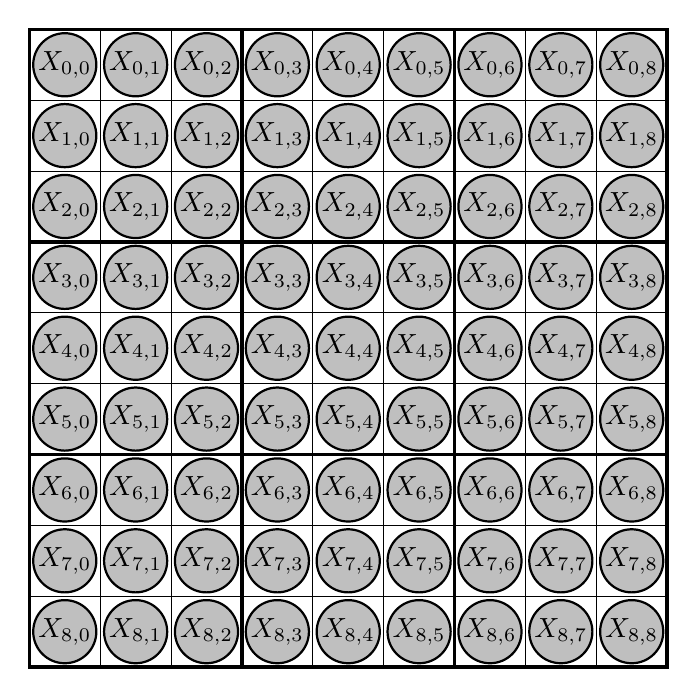
\begin{tikzpicture}[scale=0.9]
% Draw the main grid

%\node[anchor=center] (text) at (0,9) {${a)}$};

\draw[very thick] (0,0) rectangle (9,9); % Outer border
\foreach \x in {1,2,...,8} {
    \draw[thin] (\x,0) -- (\x,9); % Vertical lines
    \draw[thin] (0,\x) -- (9,\x); % Horizontal lines
}
% Thicker lines for 3x3 subgrids
\foreach \x in {3,6} {
    \draw[very thick] (\x,0) -- (\x,9); % Vertical thick lines
    \draw[very thick] (0,\x) -- (9,\x); % Horizontal thick lines
}

% Add variables in the middle of each square
\foreach \i in {0,1,...,8} {
    \foreach \j in {0,1,...,8} {
        \node[circle, draw, thick, fill=gray!50, inner sep = 0.5pt, minimum size=0.6cm, align=center] 
        at (\j+0.5,8-\i+0.5) {$X_{\i,\j}$};
    }
}

%\begin{scope}[shift={(2,0)}]
%
%\node[anchor=center] (text) at (9,9) {${b)}$};
%	
%% Draw a line of variables (horizontal)
%\foreach \k in {0,1,...,8} {
%    \node[circle, draw, thick,  fill=gray!50, inner sep=0pt, 
%    minimum size=0.6cm, align=center] 
%    at (10+\k,8.5) {$X_{i,\k}$};
%}
%
%\node[anchor=center] (text) at (9,7) {${c)}$};
%
%% Draw a column of variables (vertical)
%\foreach \l in {0,1,...,8} {
%    \node[circle, draw, thick, fill=gray!50, inner sep=0pt, 
%    minimum size=0.6cm, align=center] 
%    at (10,-\l+6) {$X_{\l,j}$};
%}
%
%\node[anchor=center] (text) at (9,7) {${d)}$};
%
%% Draw a square of variables (3x3)
%\foreach \i in {0,1,2} {
%    \foreach \j in {0,1,2} {
%        \node[circle, draw, thick, fill=gray!50, inner sep=0pt, 
%        minimum size=0.6cm, align=center] 
%        at (12+\j,6-\i) {$X_{\i,\j}$};
%    }
%}
%
%\end{scope}

\end{tikzpicture}

        \end{center}
        \caption{
            Sudoku grid of basic categorical variables $\catvariableof{i,j}$, here drawn in the standard case of $n=3$, each with dimension $\catdim=n^2=9$.
            Each basic categorical variables has $n^2$ corresponding atomization variables, which are further atomization variables to the row, column and squares constraints.
            Instead of depicting those constraints by hyperedges in a variable dependency graph, we here just indicate their existence through row, column and squares blocks.
        }\label{fig:sudokuGrid}
    \end{figure}
\end{example}




\sect{Deciding Entailment by local contractions}\label{subsec:LocalEntailment}

When having a Constraint Satisfaction Problem on a large number of variables, which are densely connected by constraint tensors, direct exploitation of the global entailment criterion in \theref{the:contCriterionLogEntailment} will be infeasible.
An alternative to deciding entailment by global operations is the use of local operations.
Here we interpret a part of the network (for example a single core) as an own knowledge base (with atomic formulas being the roots of the directed subgraph, that is potentially differing with the atoms in the global perspective) and perform entailment with respect to that.

\subsect{Monotonicity of entailment}

%\red{When defining entailment based on Markov Networks, would have clearer statement!}
Vanishing local contractions provide sufficient but not necessary criterion to decide entailment, as we show in the next theorem.

\begin{theorem}[Monotonicity of Entailment]
    \label{the:monotonEntailment}
    For any Markov Network on the decorated hypergraph $\graph$ and any subgraph $\secgraph$, we have for any formula that $\probtensor^{\graph}\models\exformula$ if $\probtensor^{\secgraph}\models\exformula$.
\end{theorem}

%To show this theorem, we show the following lemma, that whether a contraction of non-negative tensors vanishes, a vanishing contraction of a subset of these tensors is a sufficient criterion.
To prove the theorem, we first establish the following lemma that states if a contraction of non-negative tensors vanishes, the vanishing of a contraction over a subset of these tensors is a sufficient criterion.

\begin{lemma}
    \label{lem:monotocityOfVanishingContractions}
    For any non-negative tensor network $\extnet$ on $\graph$ and $\secedges\subset\edges$ we have the following.
    For $\secgraph=(\secnodes,\secedges)$ with $\secnodes=\cup_{\edge\in\secedges}\edge$ and the tensor network $\tnetof{\secgraph}$ with tensors coinciding on $\secedges$ with those in $\extnet$ we have
    \begin{align*}
        \contraction{\extnet} = 0
    \end{align*}
    if $\contraction{\tnetof{\secgraph}}=0$.
\end{lemma}
\begin{proof}
    Since the tensor network $\tnetof{\secgraph}$ is non-negative, we have whenever $\contraction{\tnetof{\secgraph}}=0$ that
    \begin{align*}
        \contractionof{\tnetof{\secgraph}}{\catvariableof{\secnodes}} = \zerosat{\catvariableof{\secnodes}} \, .
    \end{align*}
    It follows with the commutation of contractions (see \theref{the:splittingContractions} in \charef{cha:messagePassing}), that
    \begin{align*}
        \contractionof{\extnet}{\catvariableof{\nodes}}
        &= \contractionof{
            \{\hypercoreof{\edge} \, : \, \edge\in\edges/\secedges\}
            \cup \{\contractionof{\tnetof{\secgraph}}{\catvariableof{\secnodes}}\}
        }{\catvariableof{\nodes}} \\
        &=    \contractionof{
            \{\hypercoreof{\edge} \, : \, \edge\in\edges/\secedges\}
            \cup \{\zerosat{\catvariableof{\secnodes}}\}
        }{\catvariableof{\nodes}} \\
        &= 0
    \end{align*}
    Thus, also the contraction of $\extnet$ vanishes in this case.
\end{proof}

\begin{proof}[Proof of \theref{the:monotonEntailment}]
    We use \lemref{lem:monotocityOfVanishingContractions} on the subset $\tnetof{\secgraph}$ of the cores $\extnet$ to the Markov Network $\probof{\graph}$, which itself defines the Markov Network $\probof{\secgraph}$.
    Whenever $\probof{\secgraph}\models\exformula$ for a formula $\exformula$, then we have by \theref{the:contCriterionLogEntailment}
    \begin{align*}
        \contraction{\tnetof{\secgraph} \cup\{\lnot\exformula\}} = 0 \, .
    \end{align*}
    It follows with \lemref{lem:monotocityOfVanishingContractions} that also
    \begin{align*}
        \contraction{\tnetof{\graph} \cup\{\lnot\exformula\}} = 0 \, .
    \end{align*}
    and therefore $\probof{\graph}\models\exformula$.
\end{proof}


\begin{remark}
    To make use of \theref{the:monotonEntailment} we can exploit any entailment criterion.
    However, there is no general statement about entailment possible, when the local entailment does not hold.
    \theref{the:monotonEntailment} therefore just provides a sufficient but not necessary criterion of entailment with respect to $\probtensor^{\graph}$.
\end{remark}

\subsect{Knowledge Cores}

To store preliminary conclusions, we define auxiliary knowledge cores storing constraints on variables $\edge\subset\nodes$.
They are understood as logical formulas to the atomization variables $\left(\catvariableof{\edge}=\catindexof{\edge}\right)$ of the respective formulas
\begin{align*}
    \kcoreofat{\edge}{\catvariableof{\edge}}
    = \bigvee_{\catindexof{\edge} \, : \, \kcoreofat{\edge}{\indexedcatvariableof{\edge}}} \bigwedge_{\node\in\edge} \left(\catvariableof{\edge}=\catindexof{\edge}\right) \, .
\end{align*}

\begin{definition}
    Let $\extnet$ be a constraint satisfaction problem. % and $$ be a knowledge core. % \left(\catvariableof{\edge}=\catindexof{\edge}\right)
    We say that a knowledge core $\kcoreofat{\edge}{\catvariableof{\edge}}$ is sound for $\extnet$, if
    \begin{align*}
        \nonzerocirc\contractionof{\extnet}{\catvariableof{\edge}}  \prec \kcoreofat{\edge}{\catvariableof{\edge}}
    \end{align*}
    and complete for $\extnet$ if in addition
    \begin{align*}
        \nonzerocirc\contractionof{\extnet}{\catvariableof{\edge}}=\kcoreofat{\edge}{\catvariableof{\edge}} \, .
    \end{align*}
\end{definition}



\subsect{Knowledge Propagation}

\red{We now provide a solution algorithm for constraint satisfaction problems by propagating local contractions.}

Let us now draw on these insights and store partial entailment results in Knowledge Cores, which is a use of the dynamic programming paradigm.
We then iterate over local entailment checks, where we recursively add further entailment checks to be redone due to additional knowledge.
We then call the local checks until convergence Entailment Propagation, since different stadia of knowledge are propagated through the network.
We describe local Knowledge Propagation in a generic way in \algoref{alg:KnowledgePropagation}.


\begin{algorithm}[hbt!]
    \caption{Knowledge Propagation (KP)}\label{alg:knowledgePropagation}
    \begin{algorithmic}
        \State Boolean Tensor Network $\extnet$ on $\graph=(\nodes,\edges)$,
        a set of domain edges $\domainedges$
        and a set $\arbset$ of subsets of $\edges$
%	graph $\secgraph=(\nodes,\secedges)$

        \State Initialize for all $\edge\in\domainedges$:
        \begin{align*}
            \kcoreofat{\edge}{\catvariableof{\edge}}=\onesat{\catvariableof{\edge}}
        \end{align*}
        \State Initialize a queue
        \begin{align*}
            \graphqueue = \arbset
        \end{align*}
        \While{$\graphqueue$ is not empty}
            \State Choose a set of edges from the queue
            \begin{align*}
                \secedges \algdefsymbol \graphqueue\mathrm{.pop()}
            \end{align*}
            \For{$\edge\in\domainedges$ with $\edge\cap\bigcup_{\secedge\in\secedges}\secedge\neq\varnothing$}
                \State Contract
                \begin{align*}
                    \hypercoreat{\catvariableof{\edge}}
                    = \nonzerocirc\contractionof{
                        \{\hypercoreofat{\secedge}{\catvariableof{\secedge}} \, : \, \secedge\in\secedges\}
                        \cup \{\kcoreofat{\edge}{\catvariableof{\edge}} \, : \, \edge \in \domainedges , \, \edge\cap\bigcup_{\secedge\in\secedges}\secedge\neq\varnothing \}
                    }{\catvariableof{\edge}}
                \end{align*}
                \If{$\hypercoreat{\catvariableof{\edge}}\neq\kcoreofat{\edge}{\catvariableof{\edge}}$}
                    \begin{align*}
                        \kcoreofat{\edge}{\catvariableof{\edge}} \algdefsymbol \hypercoreat{\catvariableof{\edge}}
                    \end{align*}
                    \For{$\secedges\in\arbset$ with $\edge\cap\bigcup_{\secedge\in\secedges}\secedge\neq\varnothing$}
                        \begin{align*}
                            \graphqueue\mathrm{.push(}\secedges\mathrm{)}
                        \end{align*}
                    \EndFor
                \EndIf
            \EndFor
%	\State Choose $\secedge\in\secedges$ and subsets $\arbsetof{\edges}$ of $\edges$ and $\arbsetof{\secedges}$ of $\edges$  %$%of $\{\kcoreof{\edge} : \edge\in\secdges \}$ containing $\kcoreof{\edge}$
%	\State Update
%	\begin{align*}
%		\kcoreof{\secedge} \algdefsymbol\nonzerocirc\contractionof{
%			\{\hypercoreof{\edge} \, : \, \edge\in\arbsetof{\edges}\} \cup \{\kcoreof{\edge} \, : \, \edge\in\arbsetof{\secedges}\cup\{\secedge\}\}
%		}{\catvariableof{\edge}}
%	\end{align*}
        \EndWhile
    \end{algorithmic}
\end{algorithm}


%\begin{algorithm}[hbt!]
%\caption{Knowledge Propagation (KP)}\label{alg:knowledgePropagation}
%\begin{algorithmic}
%\State Boolean Tensor Network $\extnet$ on $\graph=(\nodes,\edges)$,graph $\secgraph=(\nodes,\secedges)$ with knowledge cores $\kcoreof{\edge}=\onesat{\catvariableof{\edge}}$
%\While{Stopping Criterion is not met}
%	\State Choose $\secedge\in\secedges$ and subsets $\arbsetof{\edges}$ of $\edges$ and $\arbsetof{\secedges}$ of $\edges$  %$%of $\{\kcoreof{\edge} : \edge\in\secdges \}$ containing $\kcoreof{\edge}$
%	\State Update
%	\begin{align*}
%		\kcoreof{\secedge} \algdefsymbol\nonzerocirc\contractionof{
%			\{\hypercoreof{\edge} \, : \, \edge\in\arbsetof{\edges}\} \cup \{\kcoreof{\edge} \, : \, \edge\in\arbsetof{\secedges}\cup\{\secedge\}\}
%		}{\catvariableof{\edge}}
%	\end{align*}
%\EndWhile
%\end{algorithmic}
%\end{algorithm}

% Interpretation
Each chosen subset $\secedges\in\arbset$ is understood as a local knowledge base, which is then applied for local entailment.
The knowledge cores are understood as messages, which propagate information from different regions of a tensor network (see \charef{cha:messagePassing}).


%Implementation
There are different ways of implementing \algoref{alg:knowledgePropagation}, by choosing the set $\arbset$ of constraint sets $\secedges$ and domain $\domainedges$. % and a stopping criterion.
The AC-3 algorithm (see \cite{mackworth_consistency_1977}) is a specific instance, where knowledge cores are assigned to single variables and propagation is performed on single constraint cores.


%The central property used in knowledge propagation is that any subcontraction can be added to the constraint network without changing it.
%
%\begin{theorem}\label{the:booleanContractionInvariance}
%	Given a boolean tensor network $\extnet$ on $\graph$ and $\secedges\subset\edges$.
%	For $\secgraph=(\secnodes,\secedges)$ with $\nodes=\cup_{\edge\in\secedges}\edge$ and the tensor network $\tnetof{\secgraph}$ with boolean tensors coinciding on $\secedges$ with those in $\extnet$ we have
%	\begin{align*}
%		\contractionof{\extnet}{\catvariableof{\nodes}} =
%		\contractionof{\extnet\cup\{\nonzerocirc\contractionof{\tnetof{\secgraph}}{\thirdnodes}\}}{\catvariableof{\nodes}} \, ,
%	\end{align*}
%	where $\thirdnodes\subset\nodes$ is arbitrary.
%\end{theorem}
%\begin{proof}
%	We will proof this statement later in \charef{cha:messagePassing}, see \theref{the:invarianceAddingSubcontractions}.
%\end{proof}



\begin{theorem}
    \label{the:soundnessKnowledgePropagation}
    At any state of the Knowledge Propagation \algoref{alg:knowledgePropagation}, we have that each knowledge core $\kcoreof{\secedge}$ is sound for $\extnet$.
    %\begin{align*}
    %    \contractionof{\extnet}{\nodevariables}
    %    = \contractionof{\extnet \cup \{\kcoreof{\edge} \, : \, \edge\in\domainedges\}}{\nodevariables} \, .
    %\end{align*}
    After each update in \algoref{alg:knowledgePropagation}, $\kcoreof{\secedge}$ is further monotonically decreasing with respect to the partial ordering.
    %\begin{align*}
    %    \nonzerocirc\contractionof{\extnet}{\catvariableof{\secedge}} \prec \kcoreofat{\secedge}{\catvariableof{\secedge}} \, .
    %\end{align*}
\end{theorem}
\begin{proof}
    We show the first claim by induction over the update steps in \algoref{alg:knowledgePropagation}.
    At the start, where $\kcoreofat{\edge}{\edgevariables} = \onesat{\edgevariables}$, we trivially have
    \begin{align*}
        \contractionof{\extnet \cup \{\kcoreofat{\edge}{\edgevariables} \, : \, \edge\in\domainedges\}}{\nodevariables}
        = \contractionof{\extnet \cup \{\onesat{\edgevariables} \, : \, \edge\in\domainedges\}}{\nodevariables}
        = \contractionof{\extnet}{\nodevariables} \, .
    \end{align*}
    Let us now assume, that for a state of cores $\{\kcoreof{\edge} \, : \, \edge\in\domainedges\}$ the first claim holds and let $\secedges\subset\edges$ be chosen for the update of $\kcoreof{\secedge}$.
    By the invariance under adding the support of subcontractions, which we will proof in more detail as \theref{the:monotonicityBinaryContractions} in \charef{cha:messagePassing}, we have for the update
    \begin{align*}
        \tilde{\kcore}^{\secedge}[\catvariableof{\secedge}]
        = \nonzerocirc\contractionof{
            \{\hypercoreof{\edge} \, : \, \edge\in\secedges\} \cup \{\kcoreof{\edge} \, : \, \edge\in\domainedges, \, \edge\cap\bigcup_{\secedge\in\secedges}\secedge\neq\varnothing  \}
        }{\catvariableof{\secedge}}
    \end{align*}
    that
    \begin{align*}
        \contractionof{\extnet \cup \{\kcoreofat{\edge}{\edgevariables} \, : \, \edge\in\domainedges\}}{\nodevariables}
        = \contractionof{\extnet \cup \{\kcoreofat{\edge}{\edgevariables} \, : \, \edge\in\domainedges\} \cup \{\tilde{\kcore}^{\secedge}[\catvariableof{\secedge}]\}
        }{\nodevariables}  \, .
    \end{align*}
    Thus, the first claim holds also after the update of the core to $\secedge$.

    % Since the kcore is in the contraction
    We further have with the monotonocity of boolean contraction (see \theref{the:monotonicityBinaryContractions}) that for any update of $\kcoreof{\secedge}$ by $\tilde{\kcore}^{\secedge}$
    \begin{align*}
        \tilde{\kcore}^{\secedge}[\catvariableof{\secedge}]
        = \nonzerocirc\contractionof{
            \{\hypercoreof{\edge} \, : \, \edge\in\secedges\}
            \cup \{\kcoreof{\edge} \, : \, \edge\in\domainedges, \, \edge\cap\bigcup_{\edge\in\secedges}\edge\neq\varnothing\}
        }{\catvariableof{\secedge}}
        \prec \kcoreofat{\secedge}{\catvariableof{\secedge}} \, .
    \end{align*}
    Thus, each Knowledge Core is monotoneously decreasing at each update, with respect to the partial tensor ordering.

    From the first claim we further have for any $\secedge\in\secedges$
    \begin{align*}
        \contractionof{\{\kcoreofat{\secedge}{\catvariableof{\secedge}}\}\cup\extnet \cup \left\{\kcoreof{\edge} \, : \, \edge\in\domainedges/\{\secedge\}\right\}}{\catvariableof{\secedge}}
        = \contractionof{\extnet}{\catvariableof{\secedge}}
    \end{align*}
    And thus in combination with the monotonocity of boolean contraction (see \theref{the:monotonicityBinaryContractions}) that
    \begin{align*}
        \nonzeroof{\contractionof{\extnet}{\catvariableof{\secedge}}} \prec \kcoreofat{\secedge}{\catvariableof{\secedge}}  \, .
    \end{align*}
%	We deduce the theorem from generic properties of the support of contractions, see \secref{sec:supportContractionEquations}.
%	Monotonic decreasing follows from montonocity of boolean tensor contractions, see \theref{the:monotonicityBinaryContractions}.
%	By \theref{the:invarianceAddingSubcontractions} we have during any state of the algorithm
%		\[ \nonzerocirc\contractionof{\extnet}{\catvariableof{\nodes}}  =
%		\nonzerocirc\contractionof{\extnet\cup\{\kcoreof{\edge} : \edge\in\edges\}}{\catvariableof{\nodes}}  \, .
%		\]
%	If follows that
%		\[ \nonzeroof{\contractionof{\extnet}{\edgevariables}} =  \nonzerocirc\contractionof{\extnet\cup\{\kcoreof{\edge} : \edge\in\edges\}}{\catvariableof{\edge}} \]
%	and by \theref{the:monotonicityBinaryContractions}
%		\[  \tilde{\kcoreof{\edge}}  \prec \kcoreof{\edge} \, . \]
\end{proof}


Let us now show that Knowledge Propagation always terminates.
We can further characterize the knowledge cores at termination.

\begin{definition}
    We say that a set of knowledge cores $\{\kcoreof{\edge} \, : \, \edge\in\domainedges\}$ is consistent with a set $\{\hypercoreof{\edge} \, : \, \edge\in\secedges\}$, if for any $\edge\in\domainedges$
    \begin{align*}
        \kcoreofat{\edge}{\catvariableof{\edge}}
        = \nzcontractionof{\{\hypercoreof{\edge} \, : \, \edge\in\secedges\} \cup \{\kcoreof{\edge} \, : \, \edge\in\domainedges\}}{\catvariableof{\edge}} \, .
    \end{align*}
\end{definition}

This property is similar to the completeness of a knowledge core, when interpreting the other knowledge cores and the constraints $\{\hypercoreof{\edge} \, : \, \edge\in\secedges\}$ as posing a Constraint Satisfaction Problem.

\begin{theorem}
    Knowledge Propagation \algoref{alg:knowledgePropagation} always terminates.
%    At termination, each knowledge core $\kcoreof{}$
    At termination we further for each $\secedges\in\arbset$ and $\edge\in\domainedges$ with $\edge\cap\bigcup_{\edge\in\secedges}\edge\neq\varnothing$, that the knowledge cores $\{\kcoreof{\edge} \, : \, \edge\in\domainedges, \, \edge\cap\bigcup_{\edge\in\secedges}\edge\neq\varnothing\}$ are consistent with $\{\hypercoreof{\edge} \, : \, \edge\in\secedges\}$.
\end{theorem}
\begin{proof}
    For each knowledge core, there are finitely many boolean tensor precessing it with respect to the partial order.
    Therefore, since they are monotonously decreasing, each knowledge core can only be varied finitely many times during the algorithm.
    In total the algorithm can run only finitely many times in the second for loop, where new sets of edges are pushed into the queue.
    Therefore the while loop will always terminate.

    When after a single pass through the while loop with chosen $\secedges\in\arbset$, the set $\secedges$ is not pushed back into $\graphqueue$, we have for any $\edge\in\domainedges$ with $\edge\cap\bigcup_{\edge\in\secedges}\edge\neq\varnothing$ that
%    At termination, we have for any $\secedges\in\arbset$
    \begin{align*}
        \kcoreofat{\edge}{\catvariableof{\edge}}
        = \nzcontractionof{\{\hypercoreof{\edge} \, : \, \edge\in\secedges\} \cup \{\kcoreof{\edge} \, : \, \edge\in\domainedges, \, \edge\cap\bigcup_{\edge\in\secedges}\edge\neq\varnothing\}}{\catvariableof{\edge}} \, .
    \end{align*}
    Whenever the contraction on the right hand side changes during the algorithm, the set $\secedges$ is pushed into $\graphqueue$.
    At termination of the algorithm, $\graphqueue$ is empty, and the claimed consistency therefore has to hold.
%    since otherwise the queue $\graphqueue$ would at least contain $\secedges$ and the while loop would not terminate.
\end{proof}

%A direct consequence of this theorem is that when running Knowledge Propagation with all edges, then
%\begin{corollary}
%    When we choose $\arbset=\{\edges\}$ for an CSP $\extnet$, then the knowledge cores returned by \algoref{alg:knowledgePropagation} are complete.
%\end{corollary}


We can exploit the Knowledge Propagation \algoref{alg:knowledgePropagation} for the solution of Constraint Satisfaction Problems, by taking $\extnet$ as the tensor network of constraint tensors.
Whenever a knowledge core vanishes, we can conclude that the Constraint Satisfaction Problems is not satisfiable, as we show next.

\begin{corollary}
    Let us for a Constraint Satisfaction Problem encoded by $\extnet$ run Knowledge Propagation \algoref{alg:knowledgePropagation}.
    Whenever for any $\secedge\in\edges$ we have $\kcoreofat{\secedge}{\catvariableof{\secedge}}=\zerosat{\catvariableof{\secedge}}$, then the Constraint Satisfaction Problem is not satisfiable.
\end{corollary}
\begin{proof}
    Whenever $\kcoreofat{\secedge}{\catvariableof{\secedge}}=\zerosat{\catvariableof{\secedge}}$, then we have by \theref{the:soundnessKnowledgePropagation}
    \begin{align*}
        \nonzeroof{\contractionof{\extnet}{\catvariableof{\secedge}}} \prec \zerosat{\catvariableof{\secedge}}
    \end{align*}
    and therefore
    \begin{align*}
        \contraction{\extnet} = 0 \, .
    \end{align*}
\end{proof}

% Combination with backtracking search
When the Knowledge Propagation \algoref{alg:knowledgePropagation} converges in a given implementation and no knowledge core vanishes, we can however not conclude that the Constraint Satisfaction Problem is not satisfiable.
However, for any index tuple $\catindexof{\nodes}$ to be a solution of the CSP to $\extnet$, we have the necessary condition
\begin{align*}
    \uniquantwrtof{\secedge\in\secedges}{\kcoreofat{\edge}{\catvariableof{\secedge}=\restrictionofto{\catindexof{\nodes}}{\secedges}}=1} \, ,
\end{align*}
where by $\restrictionofto{\catindexof{\nodes}}{\secedges}$ we denote the restriction of the index tuple $\catindexof{\nodes}$ to the variables included in $\secedges$.
One can use this insight as a starting point for backtracking search, where the assignments to variables $\catvariableof{\secnodes}$ are iteratively guessed, based on the restriction that each constraint is locally satisfialbe, i.e. .
\begin{align*}
    \uniquantwrtof{\secedge\in\secedges}{
        \contraction{\kcoreofat{\edge}{
            \catvariableof{\secedge\cap\secnodes}=\restrictionofto{\catindexof{\nodes}}{\secedge\cap\secnodes}
            ,\catvariableof{\secedge/\secnodes}}} \neq 0
    } \, .
\end{align*}
One can understand the guess of an assignment $\catindexof{\node}$ to a variable $\catvariableof{\node}$, as it is done during backtracking search, as an inclusion of a constraint
\begin{align*}
    \kcoreofat{\{\node\}}{\catvariableof{\node}}
    = \onehotmapofat{\catindexof{\node}}{\catvariableof{\node}} \, .
\end{align*}
Therefore, Knowledge Propagation \algoref{alg:knowledgePropagation} can be integrated with backtracking search, with iterations between propagations of knowledge and guessing of additional variables.
%The knowledge cores $\kcoreof{\edge}$ are subset encoding of possible local choices, according to which variables can be assigned.



\subsect{Applications}

Let us examplify the usage of Knowledge Propagation on Constraint Satisfaction Problems posed by entailment queries on Markov Networks.

\begin{corollary}
    \label{cor:knowledgePropagationMarkovNetworks}
    Let \algoref{alg:knowledgePropagation} be run on the cores $\tnetof{\graph}\cup\{\rencodingof{\exformula}\}$ with an arbitrary design of $\secedges$.
    Whenever for a formula $\formulaat{\catvariableof{\secnodes}}$ and a $\kcoreof{\edge}$ we have
    \[ \contractionof{\kcoreof{\edge},\rencodingof{\exformula}}{\exformulavar=0} =0  \]
    then the Markov Network $\extnet$ probabilistically entails $\exformula$.
    If on the contrary
    \[ \contractionof{\kcoreof{\edge},\rencodingof{\exformula}}{\exformulavar=1} =0  \]
    then the Markov Network $\extnet$ probabilistically entails $\lnot\exformula$, that is probabilistically contradicts $\exformula$.
\end{corollary}
\begin{proof}
    This follows from \theref{the:soundnessKnowledgePropagation} ensuring the soundness of Knowledge Propagation and the sufficiency of local entailment.
\end{proof}

\begin{example}[Batch decision of entailment]
    Let $\formulaset$ be a set of formulas and $\probofat{\graph}{\shortcatvariables}$ a Markov Network, for which it shall be decided, which formulas in $\formulaset$ are entailed, contradicted or contingent.
    We can in addition to the cores of the Markov Network create the cores $\{\rencodingofat{\exformula}{\formulavar,\shortcatvariables} \, : \, \exformula\in\formulaset\}$ and prepare the knowledge cores
    \begin{align*}
        \kcoreofat{\{\formula\}}{\formulavar} \, .
    \end{align*}
    To decide entailment batchwise, Knowledge Propagation \algoref{alg:knowledgePropagation} can be run.
    Whenever during the algorithm we have that for a $\formula$, then \corref{cor:knowledgePropagationMarkovNetworks} implies that if
    \begin{align*}
        \kcoreofat{\{\formula\}}{\formulavar} =
        \begin{cases}
            \tbasisat{\formulavar} & \text{then, the formula is entailed by }\probof{\graph} \, . \\
            \fbasisat{\formulavar} & \text{then, the formula is contradicted by }\probof{\graph} \, .\\
            \onesat{\formulavar} & \text{then no conclusion can be drawn.}
        \end{cases}
    \end{align*}
    Note, that $\kcoreofat{\{\formula\}}{\formulavar} = \zerosat{\formulavar}$ can not happen, since this would mean that $\nonzeroof{\probof{\graph}}$ is inconsistent.
    Thus, at any stage of \algoref{alg:knowledgePropagation}, one of the three holds.
    % Inference rules such as modus ponens can be mimicked.
\end{example}


\subsect{Mimiking Inference Rules by Propagation}

While so far we have discussed semantic based entailment, there are inference rules exploiting only logical syntax to infer entailed statements.
We here show, that they can be captures by the knowledge propagation scheme, if the sets $\arbset$ and $\domainedges$ are chosen properly.

Whenever
\begin{align*}
    \bigvee_{\exformula\in\formulaset} \exformula \models \secexformula
\end{align*}
then
\begin{align*}
    \tbasisat{\secexformulavar} =
    \contractionof{\{\formulaat{\shortcatvariables} \, : \, \formula\in\formulaset\} \cup \{\rencodingofat{\secexformula}{\secexformulavar,\shortcatvariables}\}}{\secexformulavar} \, ,
\end{align*}
that is the inference rule can be performed in when $\formulaset$ are in $\arbset$.

\begin{example}{Modul Ponens}
    For example, when for two formulas $\exformula,\secexformula\in\formulaset$ we have $\exformula\models\secexformula$, then when $\kcoreofat{\{\exformula\}}{\exformulavar} = \tbasisat{\formulavar}$ we have
    \begin{align*}
        \tbasisat{\secexformulavar}
        = \contractionof{(\exformula\Rightarrow\secexformula)[\exformulavar,\secexformulavar],\kcoreofat{\{\exformula\}}{\exformulavar}}{\secexformulavar} \, ,
    \end{align*}
    that is entailment of $\secexformula$ can be concluded using a single update.

    When we have a Knowledge Base of horn clauses, we run Knowledge Propagation with each horn clause being a constraint core and a knowledge core for any variable.
    \algoref{alg:knowledgePropagation} therefore resembles the forward chaining algorithm of propositional logics (see Figure~7.15 in \cite{russell_artificial_2021}).
    It is known, that forward chaining is complete for Horn Logic.
    Thus, the knowledge cores returned in that case by \algoref{alg:knowledgePropagation} are complete for the Knowledge Base as a CSP.
\end{example}


%\subsubsect{Resolution}
%Requires additional knowledge core.

% Comment
%We notice, that a careful design of \algoref{alg:knowledgePropagation} can increase the efficiency of the batchwise entailment.

\sect{Discussion}

%% Where to put?
\begin{remark}[Interpretation of Contractions in Logical Reasoning]
    The coordinates of contracted boolean tensor networks describe whether the by the coordinate indexed world is a model of the Knowledge Base at hand.
    Contractions, which only leave a part variables open, store the counts of the world respecting conditions given by the choice of slices.
    When contracting without open variables, we thus get the total world count.

    This is consistent with the probabilistic interpretation of contractions, when applying the frequentist interpretation of probability and defining normed worldcounts as probabilities.
\end{remark}


\begin{remark}{Tradeoff between generality and efficiency}
    While generic entailment decision algorithms (those by the full network) can decide any entailment, local algorithms as presented here can only perform some, but therefore more effectively as operating batchwise (dynamically deciding entailment for many leg variables).
    This is a typical phenomenon in logical reasoning and related to decidability.
\end{remark}

Local contraction approaches in inference, especially when orchestrated by a Knowledge Propagation algorithm, mimik inference rules in syntax-based prove approaches.
